\documentclass[a4paper,12pt]{article}
\usepackage[utf8]{inputenc}
\usepackage{pgfplots}
\usepackage{geometry}
\geometry{left=1in,right=1in,top=1in,bottom=1in}
\pgfplotsset{compat=1.18}
\usepgfplotslibrary{statistics}
\begin{document}

\clearpage
\begin{figure}[htbp]
\centering
\begin{tikzpicture}
\begin{axis}[width=14cm, height=9cm, xlabel={SHP Level}, ylabel={Mean Coherence}, title={Mean Coherence by SHP Level}, legend pos=outer north east, grid=major]
\addplot[black, thick] table [x=levels, y=mean_TrueCoh] {fig1_shp_data.txt}; \addlegendentry{TrueCoh}
\addplot[blue, thick] table [x=levels, y=mean_BoxCohMax] {fig1_shp_data.txt}; \addlegendentry{BoxCoh\_15}
\addplot[red, thick] table [x=levels, y=mean_AdpCoh] {fig1_shp_data.txt}; \addlegendentry{AdpCoh}
\addplot[green, thick] table [x=levels, y=mean_ModifiedCoh] {fig1_shp_data.txt}; \addlegendentry{ModifiedCoh}
\addplot[magenta, thick] table [x=levels, y=mean_BestEst] {fig1_shp_data.txt}; \addlegendentry{Best\_Est}
\end{axis}
\end{tikzpicture}
\end{figure}

\clearpage
\begin{figure}[htbp]
\centering
\begin{tikzpicture}
\begin{axis}[width=14cm, height=9cm, xlabel={SHP Level}, ylabel={Mean Coherence}, title={Mean Coherence by Box Size and SHP Level}, legend pos=outer north east, grid=major, cycle list name=color list]
\addplot[black, thick, dashed] table [x=levels, y=mean_TrueCoh] {fig2_shp_data.txt}; \addlegendentry{TrueCoh}
\addplot table [x=levels, y=BoxCoh_3] {fig2_shp_data.txt}; \addlegendentry{BoxCoh\_3}
\addplot table [x=levels, y=BoxCoh_5] {fig2_shp_data.txt}; \addlegendentry{BoxCoh\_5}
\addplot table [x=levels, y=BoxCoh_7] {fig2_shp_data.txt}; \addlegendentry{BoxCoh\_7}
\addplot table [x=levels, y=BoxCoh_9] {fig2_shp_data.txt}; \addlegendentry{BoxCoh\_9}
\addplot table [x=levels, y=BoxCoh_11] {fig2_shp_data.txt}; \addlegendentry{BoxCoh\_11}
\addplot table [x=levels, y=BoxCoh_13] {fig2_shp_data.txt}; \addlegendentry{BoxCoh\_13}
\addplot table [x=levels, y=BoxCoh_15] {fig2_shp_data.txt}; \addlegendentry{BoxCoh\_15}
\end{axis}
\end{tikzpicture}
\end{figure}

\clearpage
\begin{figure}[htbp]
\centering
% Ratio Subplot
\begin{tikzpicture}
\begin{axis}[width=14cm, height=8cm, xlabel={SHP Level}, ylabel={Coherence Ratio}, title={Ratio Estimations by SHP Level}, legend pos=outer north east, grid=major]
\addplot[black, dashed] coordinates {(1,1) (50,1)}; \addlegendentry{Reference y=1}
\addplot[blue, thick] table [x=levels, y=ratio_BoxAdp] {fig3_shp_data.txt}; \addlegendentry{Box/Adp}
\addplot[red, thick] table [x=levels, y=ratio_BoxMod] {fig3_shp_data.txt}; \addlegendentry{Box/Mod}
\addplot[green, thick] table [x=levels, y=ratio_AdpMod] {fig3_shp_data.txt}; \addlegendentry{Adp/Mod}
\end{axis}
\end{tikzpicture}

\vspace{0.5cm}

% Difference Subplot
\begin{tikzpicture}
\begin{axis}[width=14cm, height=8cm, xlabel={SHP Level}, ylabel={Coherence Difference}, title={Difference Estimations by SHP Level}, legend pos=outer north east, grid=major]
\addplot[black, dashed] coordinates {(1,0) (50,0)}; \addlegendentry{Reference y=0}
\addplot[blue, thick] table [x=levels, y=diff_BoxAdp] {fig3_shp_data.txt}; \addlegendentry{Box-Adp}
\addplot[red, thick] table [x=levels, y=diff_BoxMod] {fig3_shp_data.txt}; \addlegendentry{Box-Mod}
\addplot[green, thick] table [x=levels, y=diff_AdpMod] {fig3_shp_data.txt}; \addlegendentry{Adp-Mod}
\end{axis}
\end{tikzpicture}
\end{figure}

\clearpage
\begin{figure}[htbp]
\centering
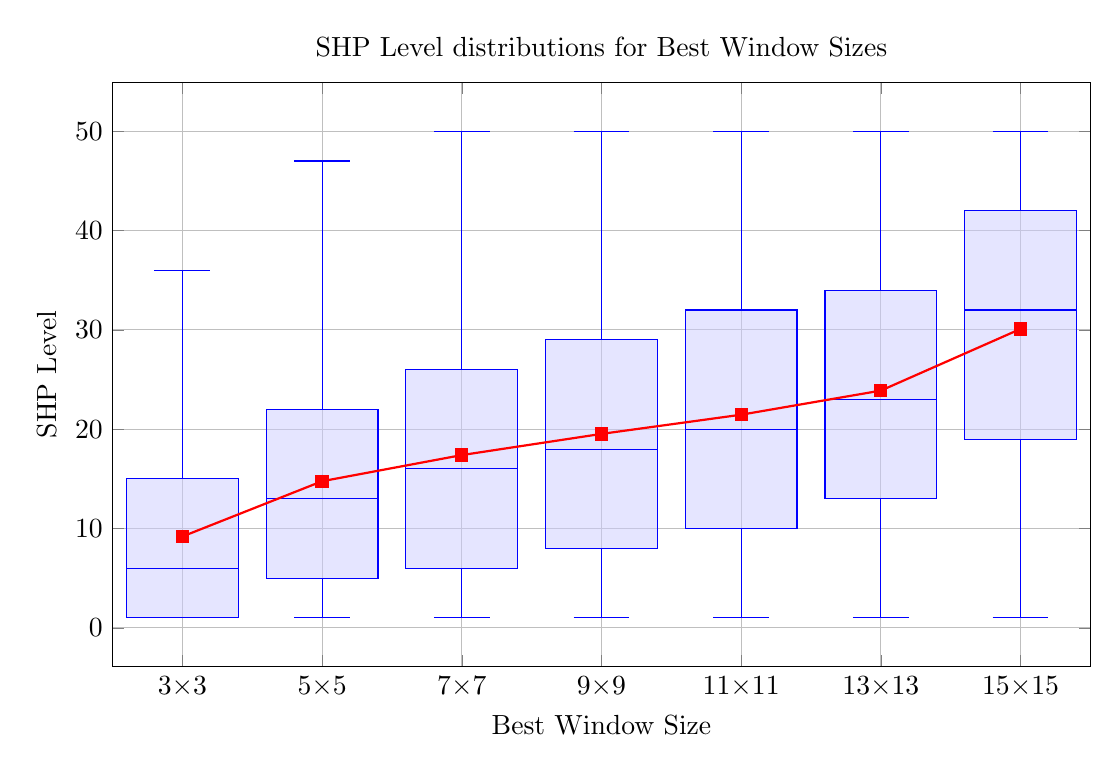
\begin{tikzpicture}
\begin{axis}[width=14cm, height=9cm, xlabel={Best Window Size}, ylabel={SHP Level}, title={SHP Level distributions for Best Window Sizes}, xtick={1,...,7}, xmin=0.5, xmax=7.5, xticklabels={3$\times$3,5$\times$5,7$\times$7,9$\times$9,11$\times$11,13$\times$13,15$\times$15}, grid=major, boxplot/draw direction=y, boxplot/whisker extend=0.4, boxplot/every whisker/.style={solid}]
\addplot+[
  boxplot prepared={
    draw position=1,
    lower whisker=1.000000,
    lower quartile=1.000000,
    median=6.000000,
    upper quartile=15.000000,
    upper whisker=36.000000,
    average=9.196898
  },
  solid, color=blue, fill=blue!20, fill opacity=0.5, mark=*
] coordinates {};
\addplot+[
  boxplot prepared={
    draw position=2,
    lower whisker=1.000000,
    lower quartile=5.000000,
    median=13.000000,
    upper quartile=22.000000,
    upper whisker=47.000000,
    average=14.762983
  },
  solid, color=blue, fill=blue!20, fill opacity=0.5, mark=*
] coordinates {};
\addplot+[
  boxplot prepared={
    draw position=3,
    lower whisker=1.000000,
    lower quartile=6.000000,
    median=16.000000,
    upper quartile=26.000000,
    upper whisker=50.000000,
    average=17.393746
  },
  solid, color=blue, fill=blue!20, fill opacity=0.5, mark=*
] coordinates {};
\addplot+[
  boxplot prepared={
    draw position=4,
    lower whisker=1.000000,
    lower quartile=8.000000,
    median=18.000000,
    upper quartile=29.000000,
    upper whisker=50.000000,
    average=19.526592
  },
  solid, color=blue, fill=blue!20, fill opacity=0.5, mark=*
] coordinates {};
\addplot+[
  boxplot prepared={
    draw position=5,
    lower whisker=1.000000,
    lower quartile=10.000000,
    median=20.000000,
    upper quartile=32.000000,
    upper whisker=50.000000,
    average=21.457830
  },
  solid, color=blue, fill=blue!20, fill opacity=0.5, mark=*
] coordinates {};
\addplot+[
  boxplot prepared={
    draw position=6,
    lower whisker=1.000000,
    lower quartile=13.000000,
    median=23.000000,
    upper quartile=34.000000,
    upper whisker=50.000000,
    average=23.884432
  },
  solid, color=blue, fill=blue!20, fill opacity=0.5, mark=*
] coordinates {};
\addplot+[
  boxplot prepared={
    draw position=7,
    lower whisker=1.000000,
    lower quartile=19.000000,
    median=32.000000,
    upper quartile=42.000000,
    upper whisker=50.000000,
    average=30.092515
  },
  solid, color=blue, fill=blue!20, fill opacity=0.5, mark=*
] coordinates {};
\addplot[color=red, thick, mark=square*] coordinates {(1, 9.196898) (2, 14.762983) (3, 17.393746) (4, 19.526592) (5, 21.457830) (6, 23.884432) (7, 30.092515) };
\end{axis}
\end{tikzpicture}
\end{figure}

\clearpage
\begin{figure}[htbp]
\centering
\begin{tikzpicture}
\begin{axis}[width=14cm, height=9cm, ybar stacked, ymin=0, ymax=100, xmin=0, xmax=51, xlabel={SHP Level}, ylabel={Percentage (\%)}, title={Best Window Size Percentage by SHP Level}, legend pos=outer north east, area legend, cycle list name=color list]
\addplot+[fill, draw=none] table [x=levels, y=Win_3] {fig5_shp_stacked.txt};
\addlegendentry{3$\times$3}
\addplot+[fill, draw=none] table [x=levels, y=Win_5] {fig5_shp_stacked.txt};
\addlegendentry{5$\times$5}
\addplot+[fill, draw=none] table [x=levels, y=Win_7] {fig5_shp_stacked.txt};
\addlegendentry{7$\times$7}
\addplot+[fill, draw=none] table [x=levels, y=Win_9] {fig5_shp_stacked.txt};
\addlegendentry{9$\times$9}
\addplot+[fill, draw=none] table [x=levels, y=Win_11] {fig5_shp_stacked.txt};
\addlegendentry{11$\times$11}
\addplot+[fill, draw=none] table [x=levels, y=Win_13] {fig5_shp_stacked.txt};
\addlegendentry{13$\times$13}
\addplot+[fill, draw=none] table [x=levels, y=Win_15] {fig5_shp_stacked.txt};
\addlegendentry{15$\times$15}
\end{axis}
\end{tikzpicture}
\end{figure}

\clearpage
\begin{figure}[htbp]
\centering
\begin{tikzpicture}
\begin{axis}[width=14cm, height=9cm, ymin=0, ymax=16, xlabel={SHP Level}, ylabel={Mean Window Size}, title={Mean Best Window Size by SHP Level}, grid=major]
\addplot[red, thick, mark=*] table [x=levels, y=mean_win_shp] {fig6_shp_mean_win.txt};
\end{axis}
\end{tikzpicture}
\end{figure}

\end{document}